\documentclass[10pt]{article}
\usepackage[utf8]{inputenc}
\usepackage[english]{babel}
\usepackage{amsmath}
\usepackage{amsfonts}
\usepackage{amssymb}
\usepackage{gensymb}
\usepackage[load=abbr]{siunitx}
\usepackage{setspace}	% for line spacing
\usepackage{calc}		% for figure scaling
\usepackage{svg}		% for graphics
\usepackage{graphicx}	% for graphics
\usepackage[left=1in,right=1in,top=1in,bottom=1in]{geometry}
\usepackage{listings}

\linespread{1.5}

% Images are build by calling images/generate.sh <images> <output> where
% output is the "build" directory used by Texmaker.
\graphicspath{{./build/images/}}
\DeclareUnicodeCharacter{2010}{ }

\author{Rob Skelly}
\title{Selection and Optimisation of Cubic Splines for Vertical Control of Remote-Sensing Unmanned Aerial Vehicles}

\lstset{%
  basicstyle=\small\ttfamily,
  language=Python
}

\begin{document}

\maketitle

\begin{abstract}
etc...
\end{abstract}

\section{Problem Statement}

In the field of remote sensing with unmanned aerial vehicles (UAVs), the flight plan is generally pre-defined using purpose-built software and followed (semi-) automonmously by the aircraft. Most currently-available software allows the creation of flight plans only in the horizontal plane \cite{AruPilot2018,DJI2018a,Microdrones2018,Group2018,UAVToolbox2018}, leaving it to the pilot to set an altitude sufficient to clear the terrain and any obstacles in the study area. Some software packages allow the selection or production of a digital elevation model (DEM) \cite{PrecisionHawk2018,UgCS2018}, but these are either tied to coarse, publicly-available datasets (which may be out of date, poorly-documented, incompatible with the working coordinate system or of doubtful provenance), or require a pre-flight and subsequent photogrammetric or LiDAR processing to produce a DEM. In either case, the resulting three-dimensional flight plan is oriented primarly towards \emph{terrain} or \emph{obstacle avoidance} rather than \emph{surface following}.

In the remote sensing context, the notion of surface following has a particular significance. The objective is not merely to avoid colliding with the terrain, but to maintain an altitude and attitude with respect to the sensed surface (which may be a vegetative canopy or the terrain itself) which preserves the quality -- image scale and distortion, point density, signal-to-noise ratio, etc. -- of the data products. Given limitations on the energy-density of current batteries, and thus flight duration, the ability to follow a trajectory safely and efficiently is also a major concern.

The present research concerns the development of a real-time, predictive, optimal flight-planning system for UAV remote sensing, to satisfy the objectives of a remote-sensing mission while resolving some of the inadequacies of existing mission-planning software packages. The system will use a forward-looking laser rangefinder to generate a two-dimensional point cloud from which a trajectory will be computed, in the form of a piecwise cubic spline. Specifically, this document proposes a rationale and procedures for selecting the type of spline (e.g., natural, constrained, weighted) and a method for parameterizing the spline to satisfy the data-quality, efficiency and safety constraints as described. 

\section{Background}

\subsection{UAV Remote Sensing}

Unmanned aerial vehicles (UAVs) are small reusable aircraft, controlled remotely by a human operator or (semi-)autonomously, which can range in size from insect-scale \cite{Avadhanula2002,Deng2003} to jet-powered military aircraft. UAVs are the subject of an explosion in engineering, scientific, military and commercial interest. Military interest in UAV research is a given, and indeed drives much of the research into the development of related technologies. Perhaps surprisingly, the development in UAVs began in 1916 and continued with the involvement of the United States military, culminating in extensive military utilization of UAVs during the war in Vietnam \cite{Valavanis2007,Cook2007}. The emergence of an entrepreneurial, just-build-it technological culture and the ability of firms to design and produce highly sophisticated, miniaturized components and high-capacity, lightweight batteries, has enabled basement tinkerers, commercial startups and academics alike exploit the capabilities offered by UAVs, rapidly and at little cost.

In particular, the availability of compact, low-power computers with high processing speeds, along with advances in real-time operating systems, have enabled the development of flight-control systems which can safely manage the inherent instability of multi-rotor aircraft. The proliferation of ``system on a chip'' (SoC) options, including environmental sensors, accelerometers, gyroscopes and magnetometers facilitiates the production of compact sensing instruments and inertial measurement units suitable for flight control. Compact, reliable laser rangefinders and spectrometers are becoming available and accessible at affordable prices. Finally, advances in battery technology are finally providing the kind of energy density and light weight that could previously be attained only with hydrocarbon fuels (and the deleterious vibration caused by reciprocating engines.) Importantly, one does not need access to electrical engineering knowledge, nor to private production facilities, to produce the sophisticated electronic hardware required for building a remote-sensing UAV. The building blocks are small enough, cheap enough and accurate enough that almost anyone can build a sensor package to their requirements.

In the scientific remote-sensing field, where the execution of an aerial survey could entail hundreds of thousands of dollars in costs for planning, permitting, instrumentation, pilots and aircraft, the advent of UAVs provides researchers with the opportunity to conduct research at much lower cost with little turnaround time. Naturally, there are compromises to be made between traditional aerial remote-sensing and the use of UAVs. UAVs tend to be limited to low altitudes, short flight durations and small site sizes. The instrumentation -- specifically multi- and hyperspectral imagers and LiDAR -- has only recently achieved a level of quality sufficient for research, and form factor small and light enough for inclusion on a UAV. Additionally, many of these instruments are designed for uses other than remote sensing, in particular LiDAR devices, which are often designed for the automotive market. However, with the drawbacks come advantages. The level of detail attainable with a low-altitude UAV survey would be impossible with a traditional aerial campaign and the cost, danger and disruption of a traditional campaign could be prohibitive.

Traditional aerial surveys have the advantage that, at typical survey altitudes of $\SI{250}\m-\SI{1000}\m$, variations in terrain relief and vegetation canopy height (collectively, surface height) are insignificant relative to the platform altitude -- except in extreme cases, such as alpine terrain -- causing minimal scale distortion in the resulting imagery. Low-altitude UAV surveys, which may take place at $\SI{10}\m-\SI{50}\m$ above the surface, encounter much larger relative variations in surface height and so must follow the surface, both to maintain the scale and quality of the data they collect, and to avoid colliding with it. In addition, because there are many structures, both natural and human-made, that may project above the the UAV's trajectory, the vehicle must have the ability to detect and avoid hazards. Manned aircraft, with an alert pilot and high altitude, rarely face such obstacles. 

The \emph{quality} of remotely-sensed data can be quantified in many ways. For example, the density of a LiDAR point cloud contributes to the power of any statistical derivatives, so the consistency of point density and accuracy across the campaign is desirable. Hyperspectral imagery can be affected by variations in atmospheric attenuation and scale distortions due to changes in platform altitude, and signal-to-noise fluctuations. As the instruments are fixed to the airframe, these characteristics must be maintained by careful management of the vehicle's velocity, altitude and attitude. In general, the lower the nominal flight elevation, for a given site, the larger the effect of surface height variation on data quality.

An important aspect of data quality is time-of-collection. A hyperspectral survey is ideally conducted as near as possible to solar noon under stable atmospheric conditions. A researcher must be opportunistic and maximise productivity during ideal conditions. Interrupting a survey to change batteries may delay the completion of the survey or limit the size of the study site, and splitting the survey over multiple days risks a change in the weather. Maximising the power efficiency of a survey, while minimizing its duration, are imperative, as is eliminating the need to repeat a survey.

The foregoing quality and efficiency concerns can be resolved, at least in part, by a terrain-following system that accurately maintains the altitude of the aircraft. Such systems are currently available but fall into two general categories: real-time altitude-control systems that use a nadir-oriented laser rangefinder to manage the aircraft's altitude \emph{reactively}, and those that require the pre-existence of a digital elevation model (DEM).

The first type of system cannot anticipate variations surface height and so has no way of optimising its trajectory to accomodate the physical limitations of the platform or data quality constraints. DEM-based terrain following systems require a high-resolution, up-to-date elevation model. If this is not available, a preliminary survey is required, meaning that at least two full surveys must be conducted, plus the processing time required to produce the model. Since the model must be produced first, the researcher has no way of knowing if conditions will still be suitable by the time the second survey is begun. A real-time terrain-following system obviates the need for these additional flights, allowing the researcher to conduct surveys during ideal conditions as they arise, and to adapt the flight plan in real-time to accomodate the prevailing conditions.

Any terrain-following system must be able to accomodate the different surface charactistics and mission objectives that a researcher may encounter. For example, a vineyard's rows (figure \ref{fig:photo_culmina_rows}) are spaced roughly $\SI{2}\m$ apart, creating a depression between rows. It would be undesireable for the aircraft to descend into the spaces between rows; rather, its trajectory should carry it smoothly over a surface implied by the tops of the rows while it follows the low-frequency variations in the surface (fgure \ref{fig:photo_culmina_rows_slope}). In this sense, a terrain-following system is a low-pass filter with configurable sensitivity.

\begin{figure} %[htbp] % htbp stand for "here", "top", "bottom", "page"
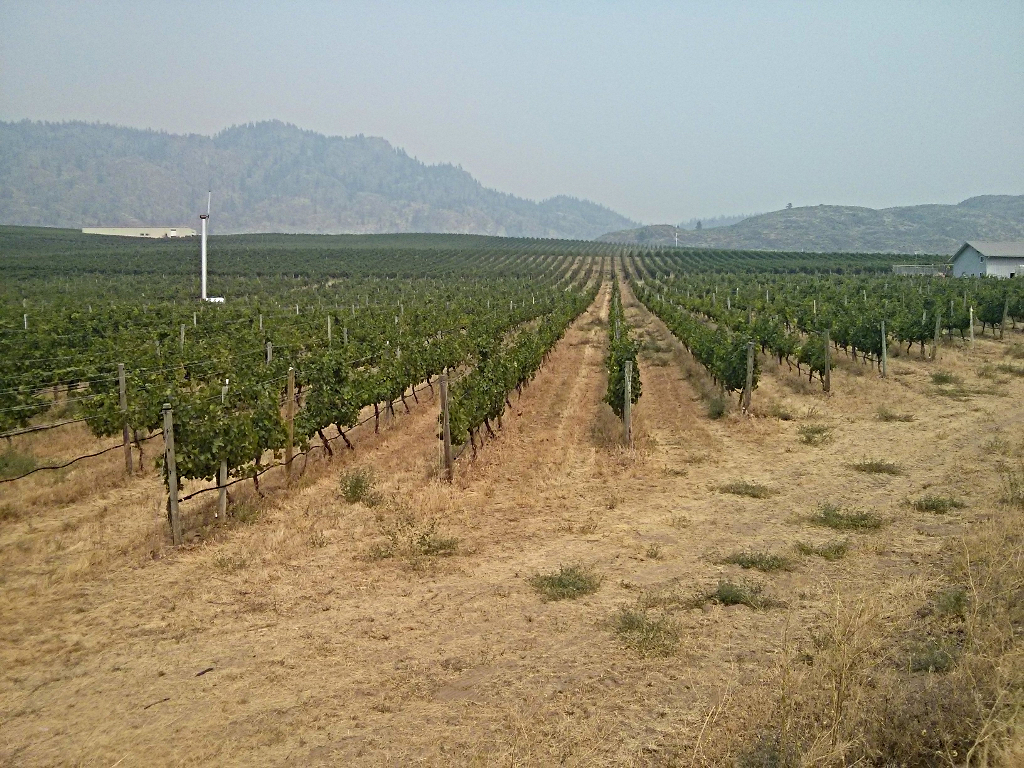
\includegraphics[width=1.0\linewidth]{tmp/photo_culmina_rows.pdf} 
\caption{Typical spacing of vinyard rows. Culmina Winery, Penticton, BC. August 2017.}
\label{fig:photo_culmina_rows}
\end{figure}

\begin{figure} %[htbp] % htbp stand for "here", "top", "bottom", "page"
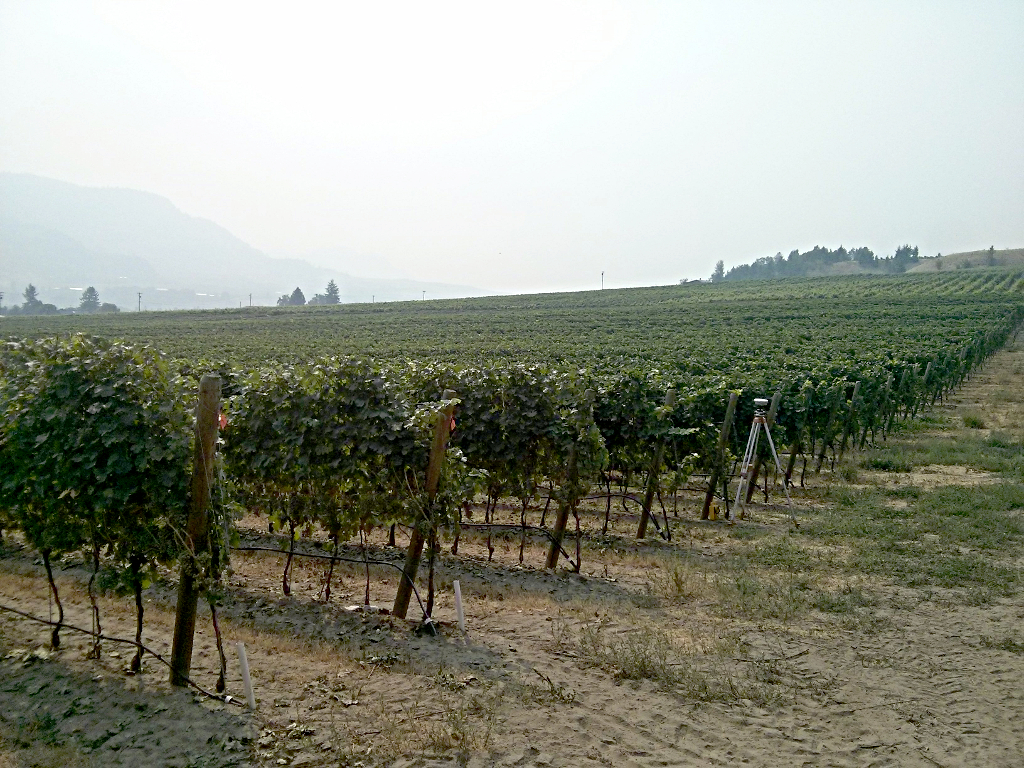
\includegraphics[width=1.0\linewidth]{tmp/photo_culmina_rows_slope.pdf} 
\caption{Low-frequency surface height variation, Culmina Winery, Penticton, BC. August 2017.}
\label{fig:photo_culmina_rows_slope}
\end{figure}

In the foregoing instances, a regular pattern of variation prevails, but there are other environments that may confuse a system configured for these conditions. The subalpine regions of Canada's West Coast demonstrate multi-scale variability, incoroporating smooth meadow-like environments, highly-variable multiple-aged forest canopies, and large-scale, high-relief terrain (figure \ref{fig:photo_san_juan}).

\begin{figure} %[htbp] % htbp stand for "here", "top", "bottom", "page"
\begin{center}
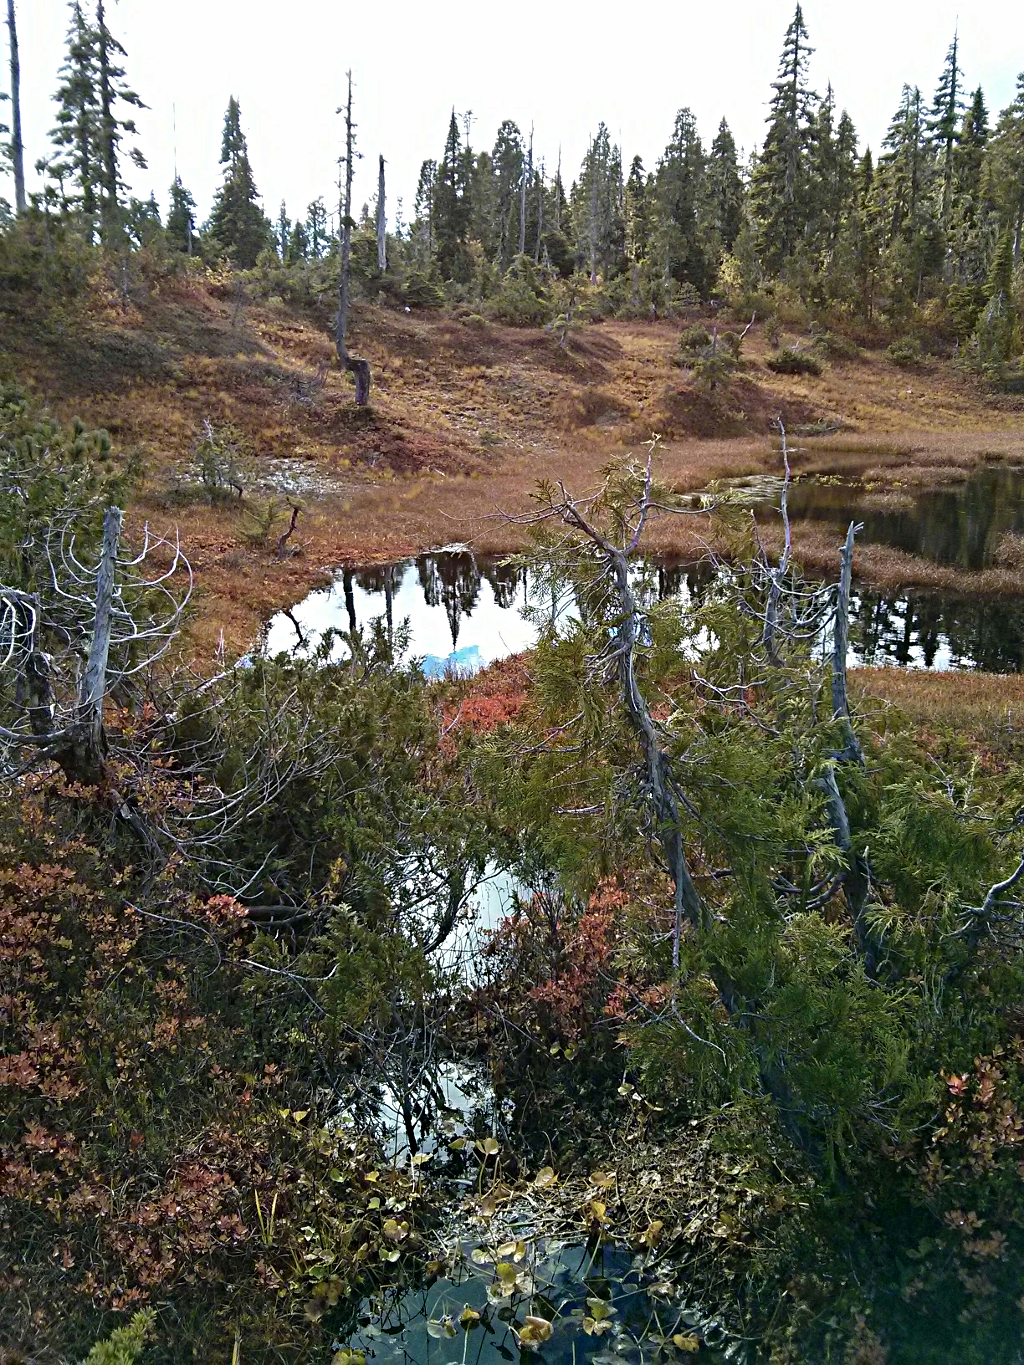
\includegraphics[width=0.5\linewidth]{tmp/photo_san_juan.pdf} 
\end{center}
\caption{Variable-frequency surface height variation in a subalpine environment, San Juan Ridge, BC. October 2014.}
\label{fig:photo_san_juan}
\end{figure}



\subsection{Cubic Splines}

The word "spline" originates in construction, where long, flexible wooden beams, called splines, were used to model curves. Splines have a tendency, when held at two or more points, called "ducks," to seek a shape which minimizes stored energy in the beam. As such, the spline could be considered an optimal interpolator \cite{Wegman2016}. In mathematics, the spline is usually represented by piecewise cubic polynomials, one for each pair of ducks, or \emph{knots}, distinguished by the permissible dicontinuities at the ends. The minimum-energy constraint is modelled by minimizing mean square curvature of the polynomial \cite{Wegman2016}.

The mechanical spline is, of course, an interpolator -- it passes through each of the "ducks." At

The constraints placed on the spline's ends determine the type of spline. In a "free" spline, the ends are free to assume any angle. In a "natural" spline, the ends are held at a specific angle. 

In mathematics, the spline is an attempt to model this physical behaviour. 





The purpose of this research is to develop a forward-looking, predictive, terrain-following system for the control of unmanned aerial vehicles for remote sensing. 


In this instance, the distance to the surface is measured using a LightWare SF30/C laser rangefinder mounted on a scanning d





\newpage
\bibliographystyle{plain}
\bibliography{/home/rob/Documents/bibtex/library}

\end{document}